%%%%%%%%%%%%%%%%%%%%%%%%%%%%%%%%%%%%%%%%%
% Seismica Submission Template
%%%%%%%%%%%%%%%%%%%%%%%%%%%%%%%%%%%%%%%%%

%% Options available: 
%%					anonymous
%%					breakmath
%%					languages
%%					preprint
%%					report

%% anonymous: produces an anonymous PDF for double-blind review. Will NOT print authors information and acknowledgements, but WILL PRINT data availibility section, so be careful!
%% breakmath: for manuscripts with many long formulas, you can specify the breakmath option (loads the package breqn and uses the dmath environment)
%% languages: see below, use to add abstract(s) in additional languages
%% preprint: removes line numbers, switch to two-columns
%% report: if this is a report

%\documentclass[breakmath,report]{seismica}
\documentclass[]{seismica}
% subfig and subcaption are mutually incompatible; keep only subcaption.
\usepackage{subcaption}
% Network DOIs contain underscores; detokenize the printed DOI (hyperref handles
% the underscore in the URL) so \doi{...} in the bibliography does not error.
\AtBeginDocument{\renewcommand{\doi}[1]{\href{https://doi.org/#1}{doi:\detokenize{#1}}}}

\title{Supplementary Materials} % used for header, not mandatory
% other titles From Picks to Catalog: Ensemble Deep Learning and Graph Networks Map Cascadia’s Quiet Megathrust


%% If this is a REPORT, select a report type within: 
%\reporttype{Null Results Report} % (null-results/failed experiments)
%\reporttype{Software Report}
%\reporttype{Data Report} %  (e.g., Large Community dataset initiatives, Instrument Deployments, and Field Campaigns)
\reporttype{Fast Report}

%% Will not be printed if anonymous option ON



\author[1]{Marine~Denolle
\orcid{0000-0002-1610-2250}
\thanks{Corresponding author: mdenolle@uw.edu}
}


\author[1]{Hiroto Bito
\orcid{0009-0001-4138-0287}
}
\author[1]{Qibin~Shi
\orcid{2222-2222-2222-2222}
}
\author[1]{Yiyu~Ni
\orcid{3333-3333-3333-3333}
}

\author[2]{Ian W. McBrearty
\orcid{3333-3333-3333-3333}
}

\author[3]{Zoe~Krauss
\orcid{3333-3333-3333-3333}
}
\author[4]{Nathan T. Stevens
\orcid{0000-0001-5648-2254}
}

\author[2]{Yifan Yu
\orcid{0000-0001-5986-9702}
}

\author[2]{Gregory C.~Beroza
\orcid{3333-3333-3333-3333}
}



\affil[1]{Department of Earth and Space Sciences, University of Washington, Seattle, USA}
\affil[2]{Department of Geophysics, Stanford University, USA}
\affil[3]{School of Oceanography, University of Washington, Seattle, USA}
\affil[4]{Pacific Northwest Seismic Network, University of Washington, Seattle, USA }

%% Author CRediT roles 
%% Please use the CRediT roles as defined at https://casrai.org/credit
%% Use as many roles as necessary; there is no requirement to use all 14 roles
\credit{Conceptualization}{Name Firstauthor, Name Thirdauthor}
%\credit{Methodology}{people}
%\credit{Software}{people}
%\credit{Validation}{people}
\credit{Formal Analysis}{Name Firstauthor, Name Secondauthor}
%\credit{Investigation}{people}
%\credit{Resources}{people}
\credit{Writing - Original draft}{Name Firstauthor}
%\credit{Writing - Review \& Editing}{people}
%\credit{Visualization}{people}
%\credit{Supervision}{people}
%\credit{Project administration}{people}
%\credit{Funding acquisition}{people}


%%%%%%%%%%%%%%%%%%%%%%%%%%%%%%%%%%%%%%%%%
%% Abstracts in other languages
%%%%%%%%%%%%%%%%%%%%%%%%%%%%%%%%%%%%%%%%%
%% If your article includes abstracts in other languages, uncomment the lines below and fill in
%%      the appropriate sections. You will need to use the [languages] option at the top,
%%      and will need to use lualatex instead of pdflatex to compile the document.
%% We will use luatex, polyglossia and fontspec for the compilation of the accepted version. 
%% Feel free to use any polyglossia command.
%\setotherlanguages{french,thai}  % replace with your language(s), per polyglossia
%% if an additional font is needed for the abstract, load it with:
%\newfontfamily\thaifont[Script=Thai]{Noto Serif Thai}

%% If you are using Arabic, do not include it in \setotherlanguages{} as it is not supported 
%% by polyglossia. Instead, with the [languages] option at the top, you can use these commands
%% within the text:
%%\begin{Arabic} and \end{Arabic} around paragraphs in Arabic
%%\n{} to wrap any digits within Arabic text that should read left-to-right
%%\textarabic{} for Arabic text embedded in a left-to-right paragraph

%% also see https://www.overleaf.com/latex/examples/how-to-write-multilingual-text-with-different-scripts-in-latex/wfdxqhcyyjxz for reference
%%%%%%%%%%%%%%%%%%%%%%%%%%%%%%%%%%%%%%%%%

%%%%%%%%%%%%%%%%%%%%%%%%%%%%%%%%%%%%%%%%%
%% Several abstracts
%%%%%%%%%%%%%%%%%%%%%%%%%%%%%%%%%%%%%%%%%
%% the command \makeseistitle does not allow page breaks in preprint mode. If you have
%%		many abstracts, you can use the command \addsummaries. It will induce a pagebreak.

\begin{document}

%% Your article can include up to 3 abstracts. The first is the English language abstract.
%% For other languages in the second and third optional abstracts, you might have to define 
%%      additional font(s) in preamble above
%% You can also include a non-technical summary in addition to the abstract(s)
\makeseistitle{
    \begin{summary}{Abstract}
blablba
           \end{summary}
}  %% don't forget this one!


\section{Alternative Workflow}


The geographic region of the subject is the following: the latitude ranges from  40°–50° N and longitude ranges from 122°–129° W. The P and S phases from the region were picked with the Ensemble Learning Earthquake Prediction (ELEP) framework \citep{Yuan23}. 
All the stations in the following networks are attempted to be used to pick the phases: C8, 7D, 7A, CN, NV, UW, UO, NC, BK, TA, OO, PB, X6, Z5, and X9. The picks were obtain from 2010 to 2015.

\subsection{Phase Picking}

The semblance-based ensemble method was used \citep{Yuan23}. There are two formats of the pick data frames. The first format resembles the Seisbench format (cite). The second format was developed in the project. The picks are saved in a file for a single station and date. The pick files are then merged into a single file. The merged file contains 39597551 picks. A data frame with station metadata were compiled using the merged file. The data frame of station metadata contains information of 453 stations. 

\subsection{Phase Association}
Association was conducted in 10 different subregions across the CSZ. The 10 subregions were defined by the 10 different sets of nodes that are prepared base on the node information provided by \citet{Stone18}. Each set of nodes has a velocity model assigned to it \citep{Yuan23}.

Each node has an inner circle and an outer circle (REF3). The information of a node includes the latitude and longitude of the center of the node, the radial distance from the center to the inner circle and the radial distance from the inner circle to the outer circle (Klein, 2019; Stone et al., 2018). 
Oregon: Shelf and Trench uses the depths and the velocity profile of the P phase from Oregon: Shelf (Stone et al., 2018). Similarly, Southern Washington: Shelf and Trench uses the depths and the velocity profile of the P phase from Southern Washington: Shelf (Stone et al., 2018). Lastly, Northern Washington: Shelf and Trench uses the depths and the velocity profile of the P phase from Northern Washington: Shelf (Stone et al., 2018). 

The station ID and location information of the stations that fall within the outer circle of each subregion was saved in a data frame specific to the subregion (Klein, 2019; Stone et al., 2018). Each subregion has picks from stations that are located in the subregion. Those picks were obtained from the merged pick file using the station ID’s in the above-mentioned station data frame (Klein, 2019; Stone et al., 2018). 
For each subregion, the pick data frame and the station data frame were inputted to the associator to produce the event and assignment tables (REF4). The event table was populated with the the pick information by merging with the assignment table (REF4).

\subsection{Location}

The merged assignment tables of the 10 subregions were merged together to make a single assignment table. 

\subsection{Results}

\subsection{Discussion}

\section{Depth resolution and tectonic setting}

Focal depth is solved (not fixed) but constrained only moderately by the
ocean-bottom geometry: about half the quality-controlled catalog is well determined
(azimuthal gap $<180^\circ$, $\ge 6$ S picks, positive depth). Figure~\ref{fig:supp_depth}
separates that well-constrained subset. Deformation-front events peak in the upper
crust ($\sim$13~km); forearc and arc events cluster at $\sim$18--20~km. The offshore
ridge/transform events are scattered and biased deep because they lie west of the
array (large gaps), so their depths are the least reliable. In the forearc
cross-section, the abundant seismicity at 10--20~km sits well \emph{above} the Slab2
subduction interface (which deepens landward from $\sim$9~km to $\sim$50~km), indicating
predominantly crustal, upper-plate seismicity rather than events on the largely locked
megathrust.

\begin{figure}[h]
    \centering
    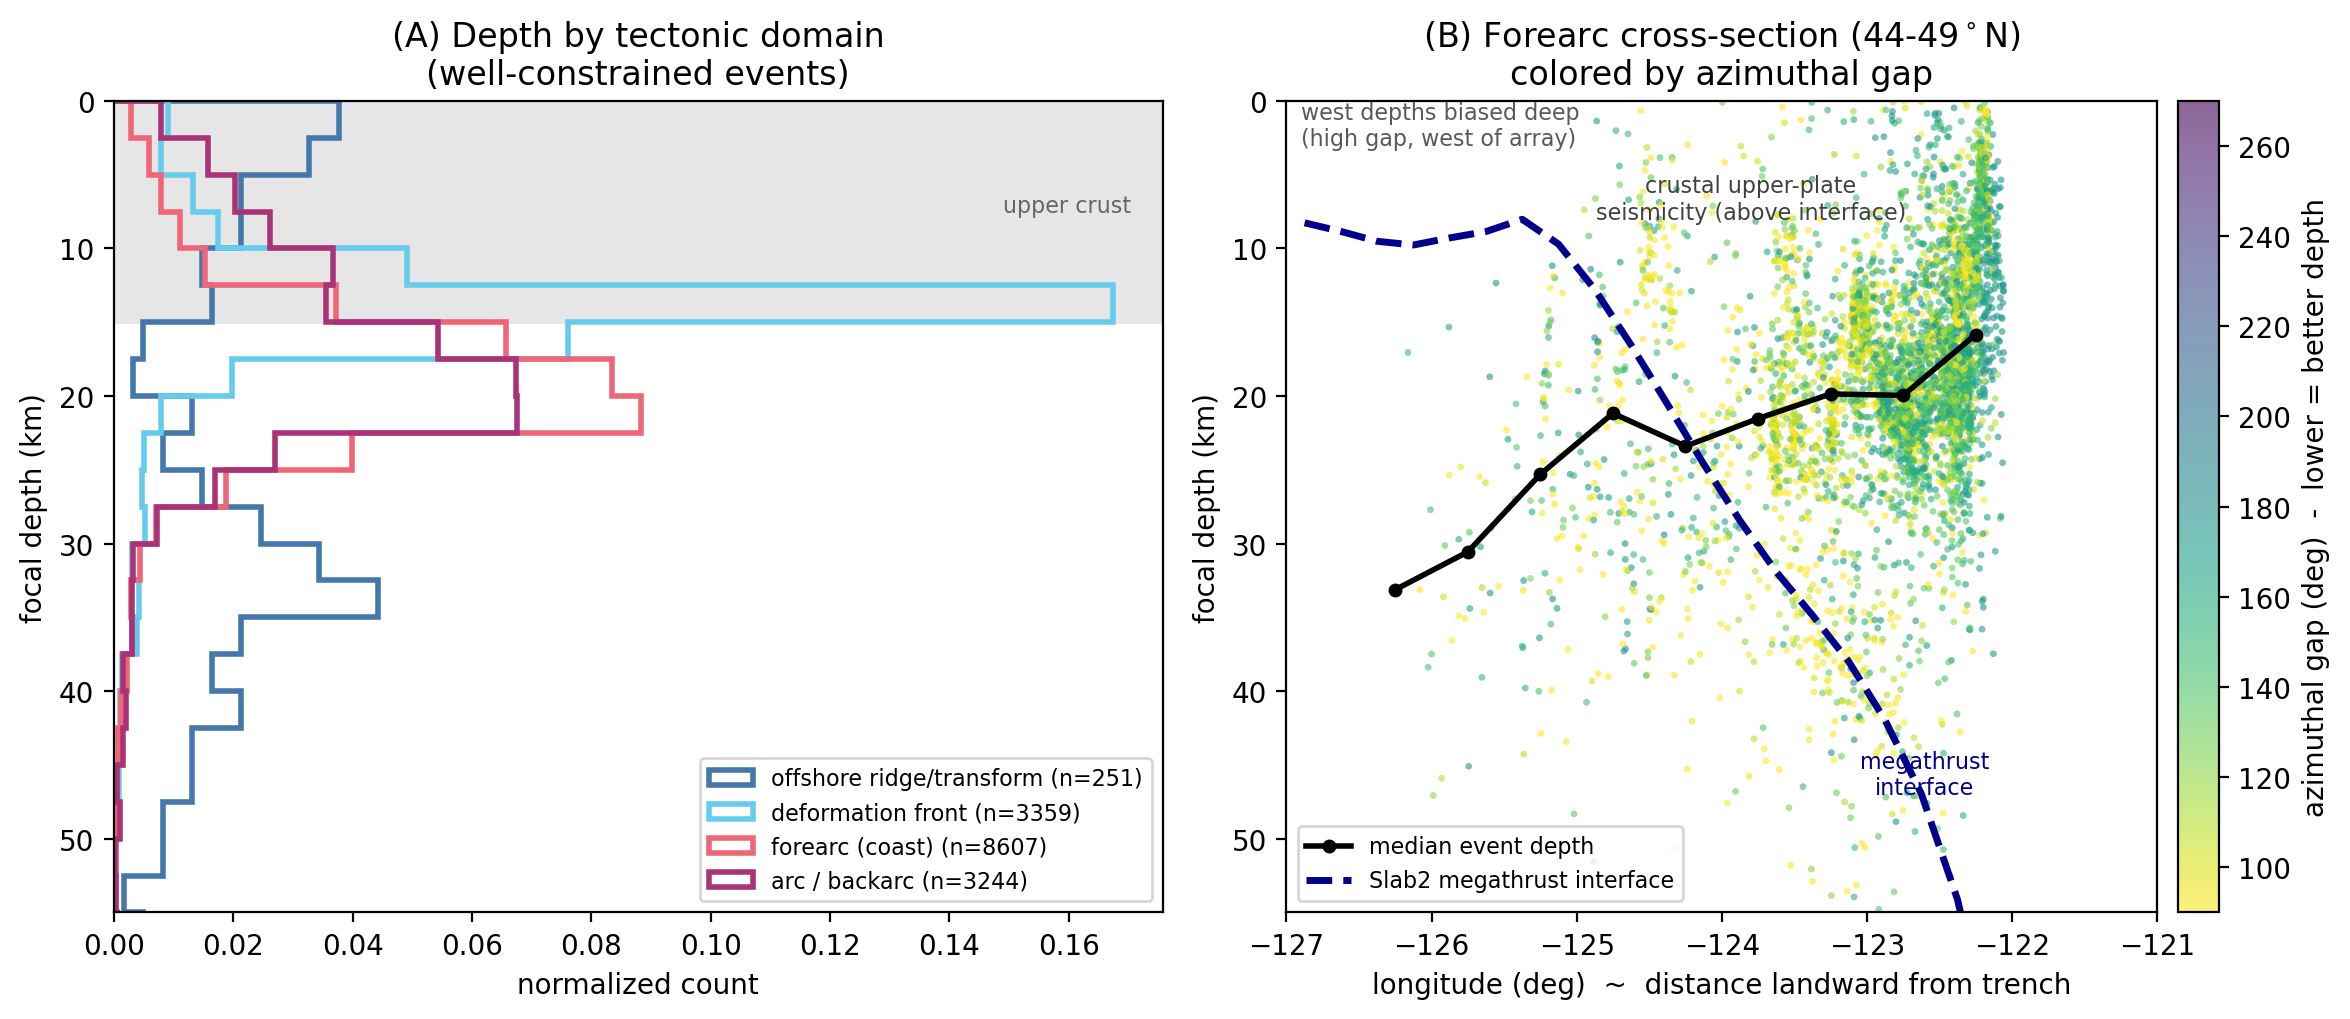
\includegraphics[width=\linewidth]{figures/supp_depth_analysis.png}
    \caption{{\bf Depth structure.} (a) Depth distributions by tectonic domain
    (well-constrained events). (b) Forearc longitude--depth cross-section
    (44--49$^\circ$N) colored by azimuthal gap, with the Slab2 megathrust interface
    (dashed). The apparent westward-deepening of median depth is a network-geometry
    artifact (offshore events biased deep); most forearc seismicity is crustal,
    above the interface.}
    \label{fig:supp_depth}
\end{figure}

\section{A generous megathrust bucket}

Given the combined uncertainty of the plate-interface geometry and of our focal
depths, we bound how much of the catalog \emph{could} be megathrust-related rather
than asserting which events are. An event is placed in a generous bucket when its
depth lies within the Slab2 model's own vertical uncertainty at that location
\citep[cas\_slab2\_unc; median $\sim$13~km for Cascadia, larger offshore;][]{Hayes18}
plus a small margin for our relocation depth error and for the few-kilometre offsets
that newer offshore imaging finds relative to Slab2. This upper bound is
$\sim$44\% of the catalog (Figure~\ref{fig:supp_bucket}); it forms a coherent band
along the deformation front and lower forearc, whereas the abundant shallow inland
seismicity falls above the interface (crustal upper plate) and the offshore
ridge/transform events fall outside the modeled slab. The bucket is an upper limit:
most of these events are equally consistent with crustal or intraslab faulting given
the depth resolution.

\begin{figure}[h]
    \centering
    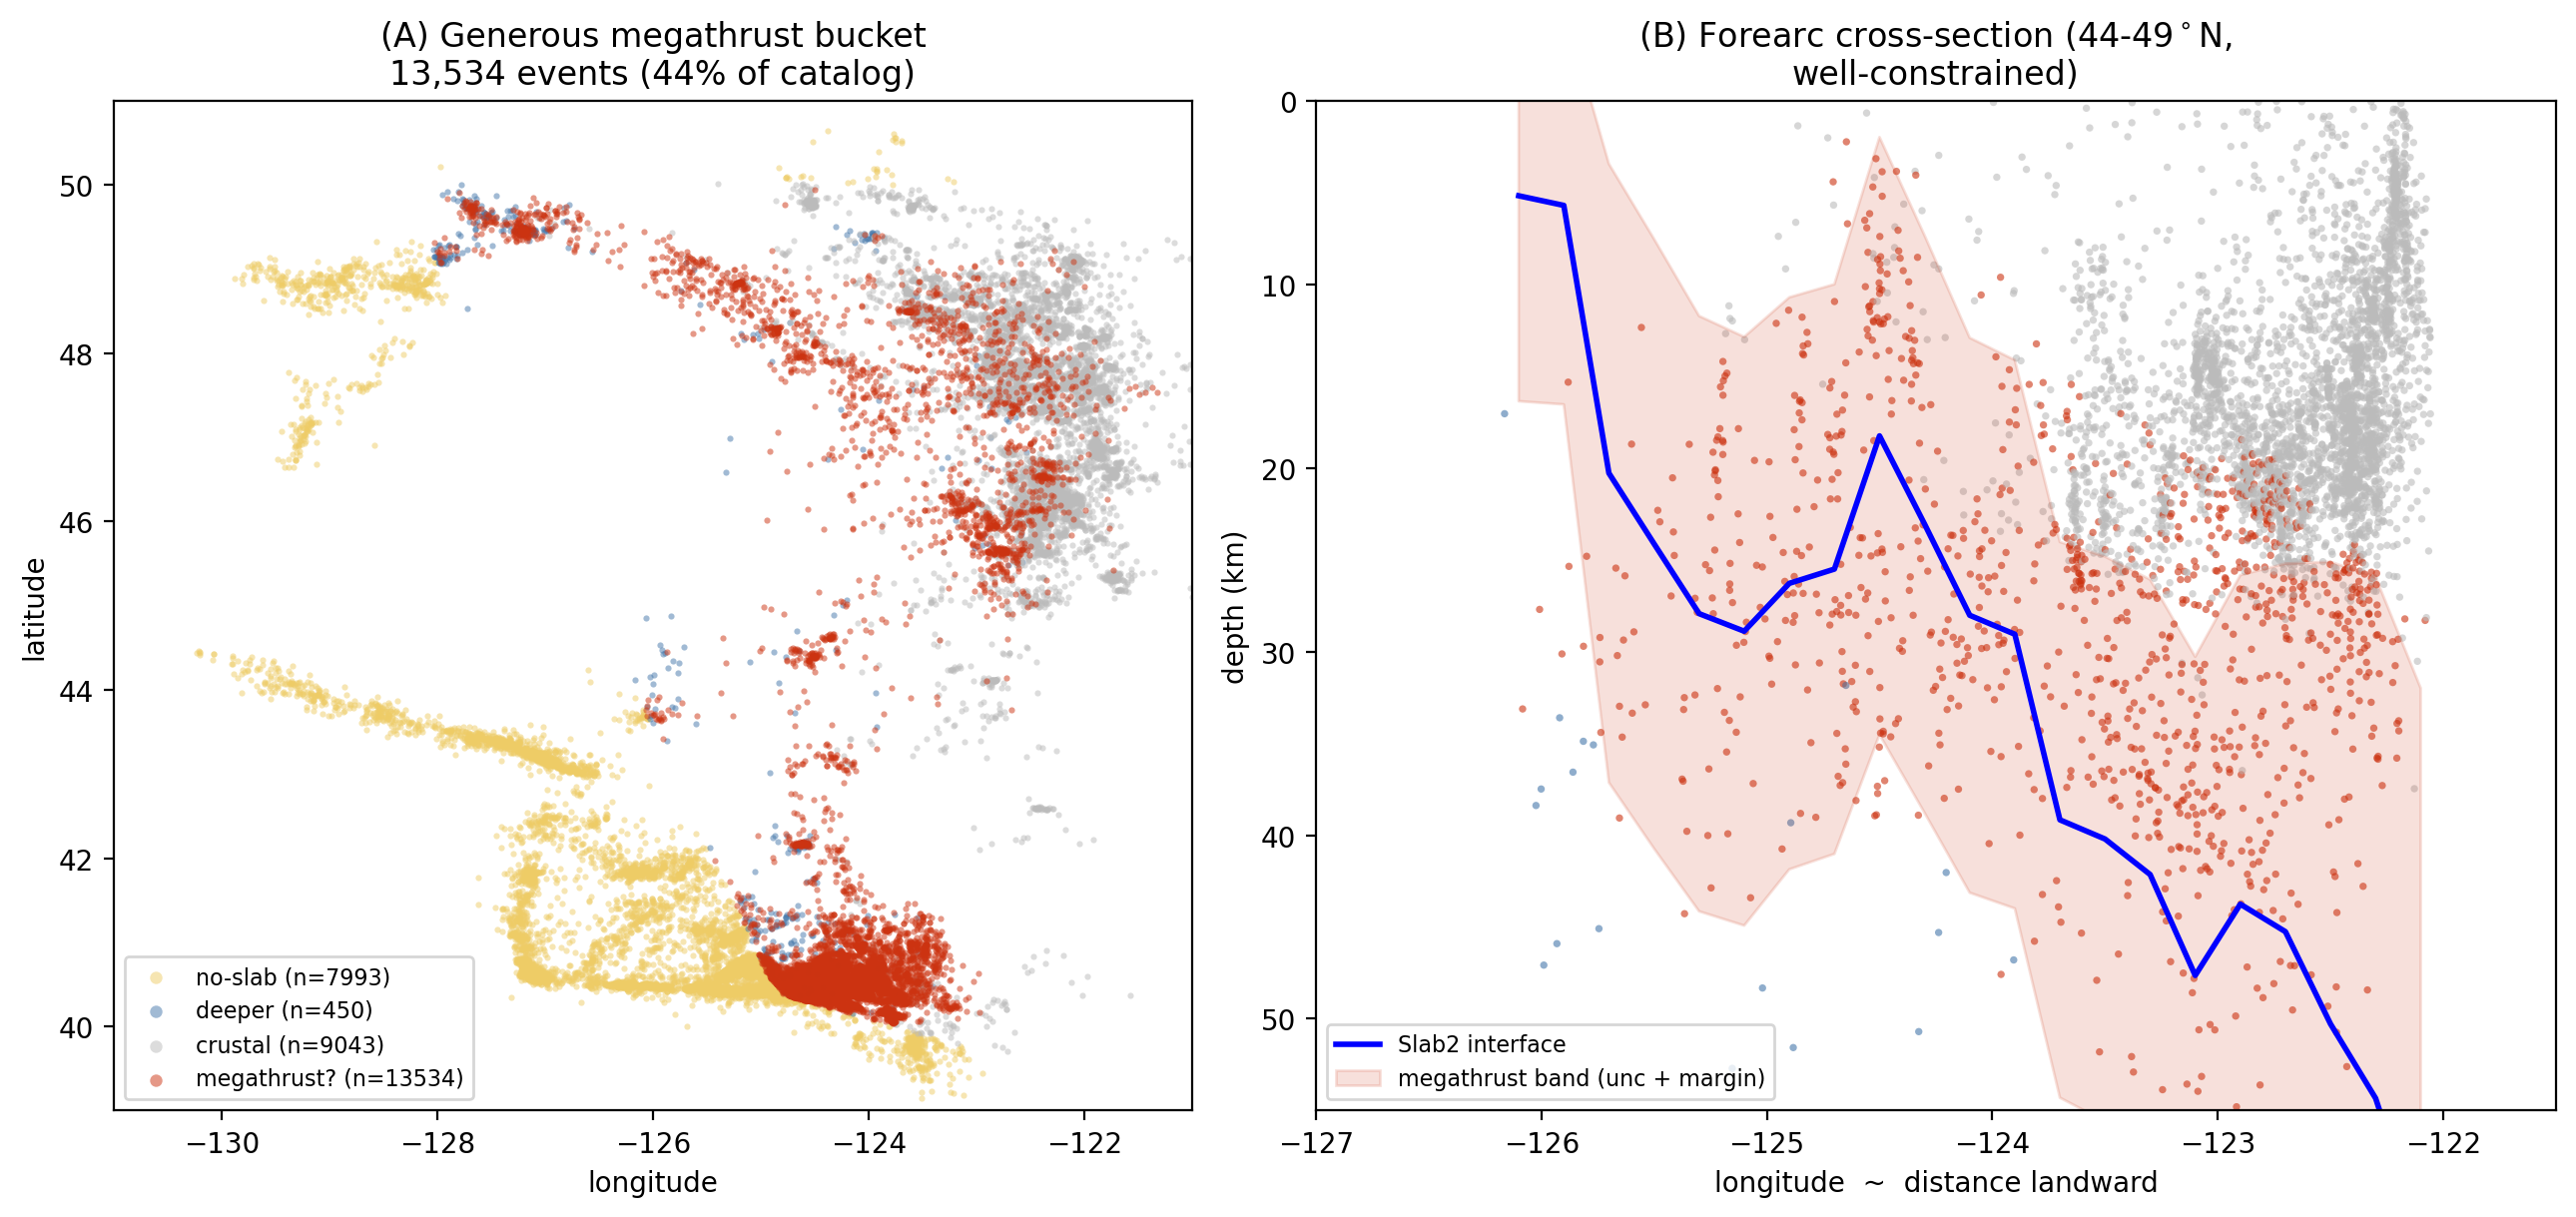
\includegraphics[width=\linewidth]{figures/supp_megathrust_bucket.png}
    \caption{{\bf Generous megathrust bucket.} (a) Map of quality-controlled events
    classified against the Slab2 interface $\pm$(uncertainty $+$ margin): potentially
    megathrust (red), crustal/above (grey), intraslab/below (blue), and no modeled
    slab beneath (yellow; ridge/transform). (b) Forearc cross-section with the Slab2
    interface and its generous uncertainty envelope.}
    \label{fig:supp_bucket}
\end{figure}

\section{Temporal context and coverage}

Figure~\ref{fig:supp_temporal} places the catalog in time. Monthly seismicity runs
largely independently of the tectonic-tremor (ETS) cycle, as expected for
upper-plate/intraslab seismicity, and the offshore detection rate grows as the
Cascadia-Initiative OBS array is deployed. The offshore latitude--time distribution
exposes a coverage gap along the central Juan de Fuca ridge and Axial Seamount
($\sim$45--46.6$^\circ$N): no events are recovered there across the whole period,
including through the April 2015 Axial eruption, a domain monitored by the OOI cabled
array rather than these OBS.

\begin{figure}[h]
    \centering
    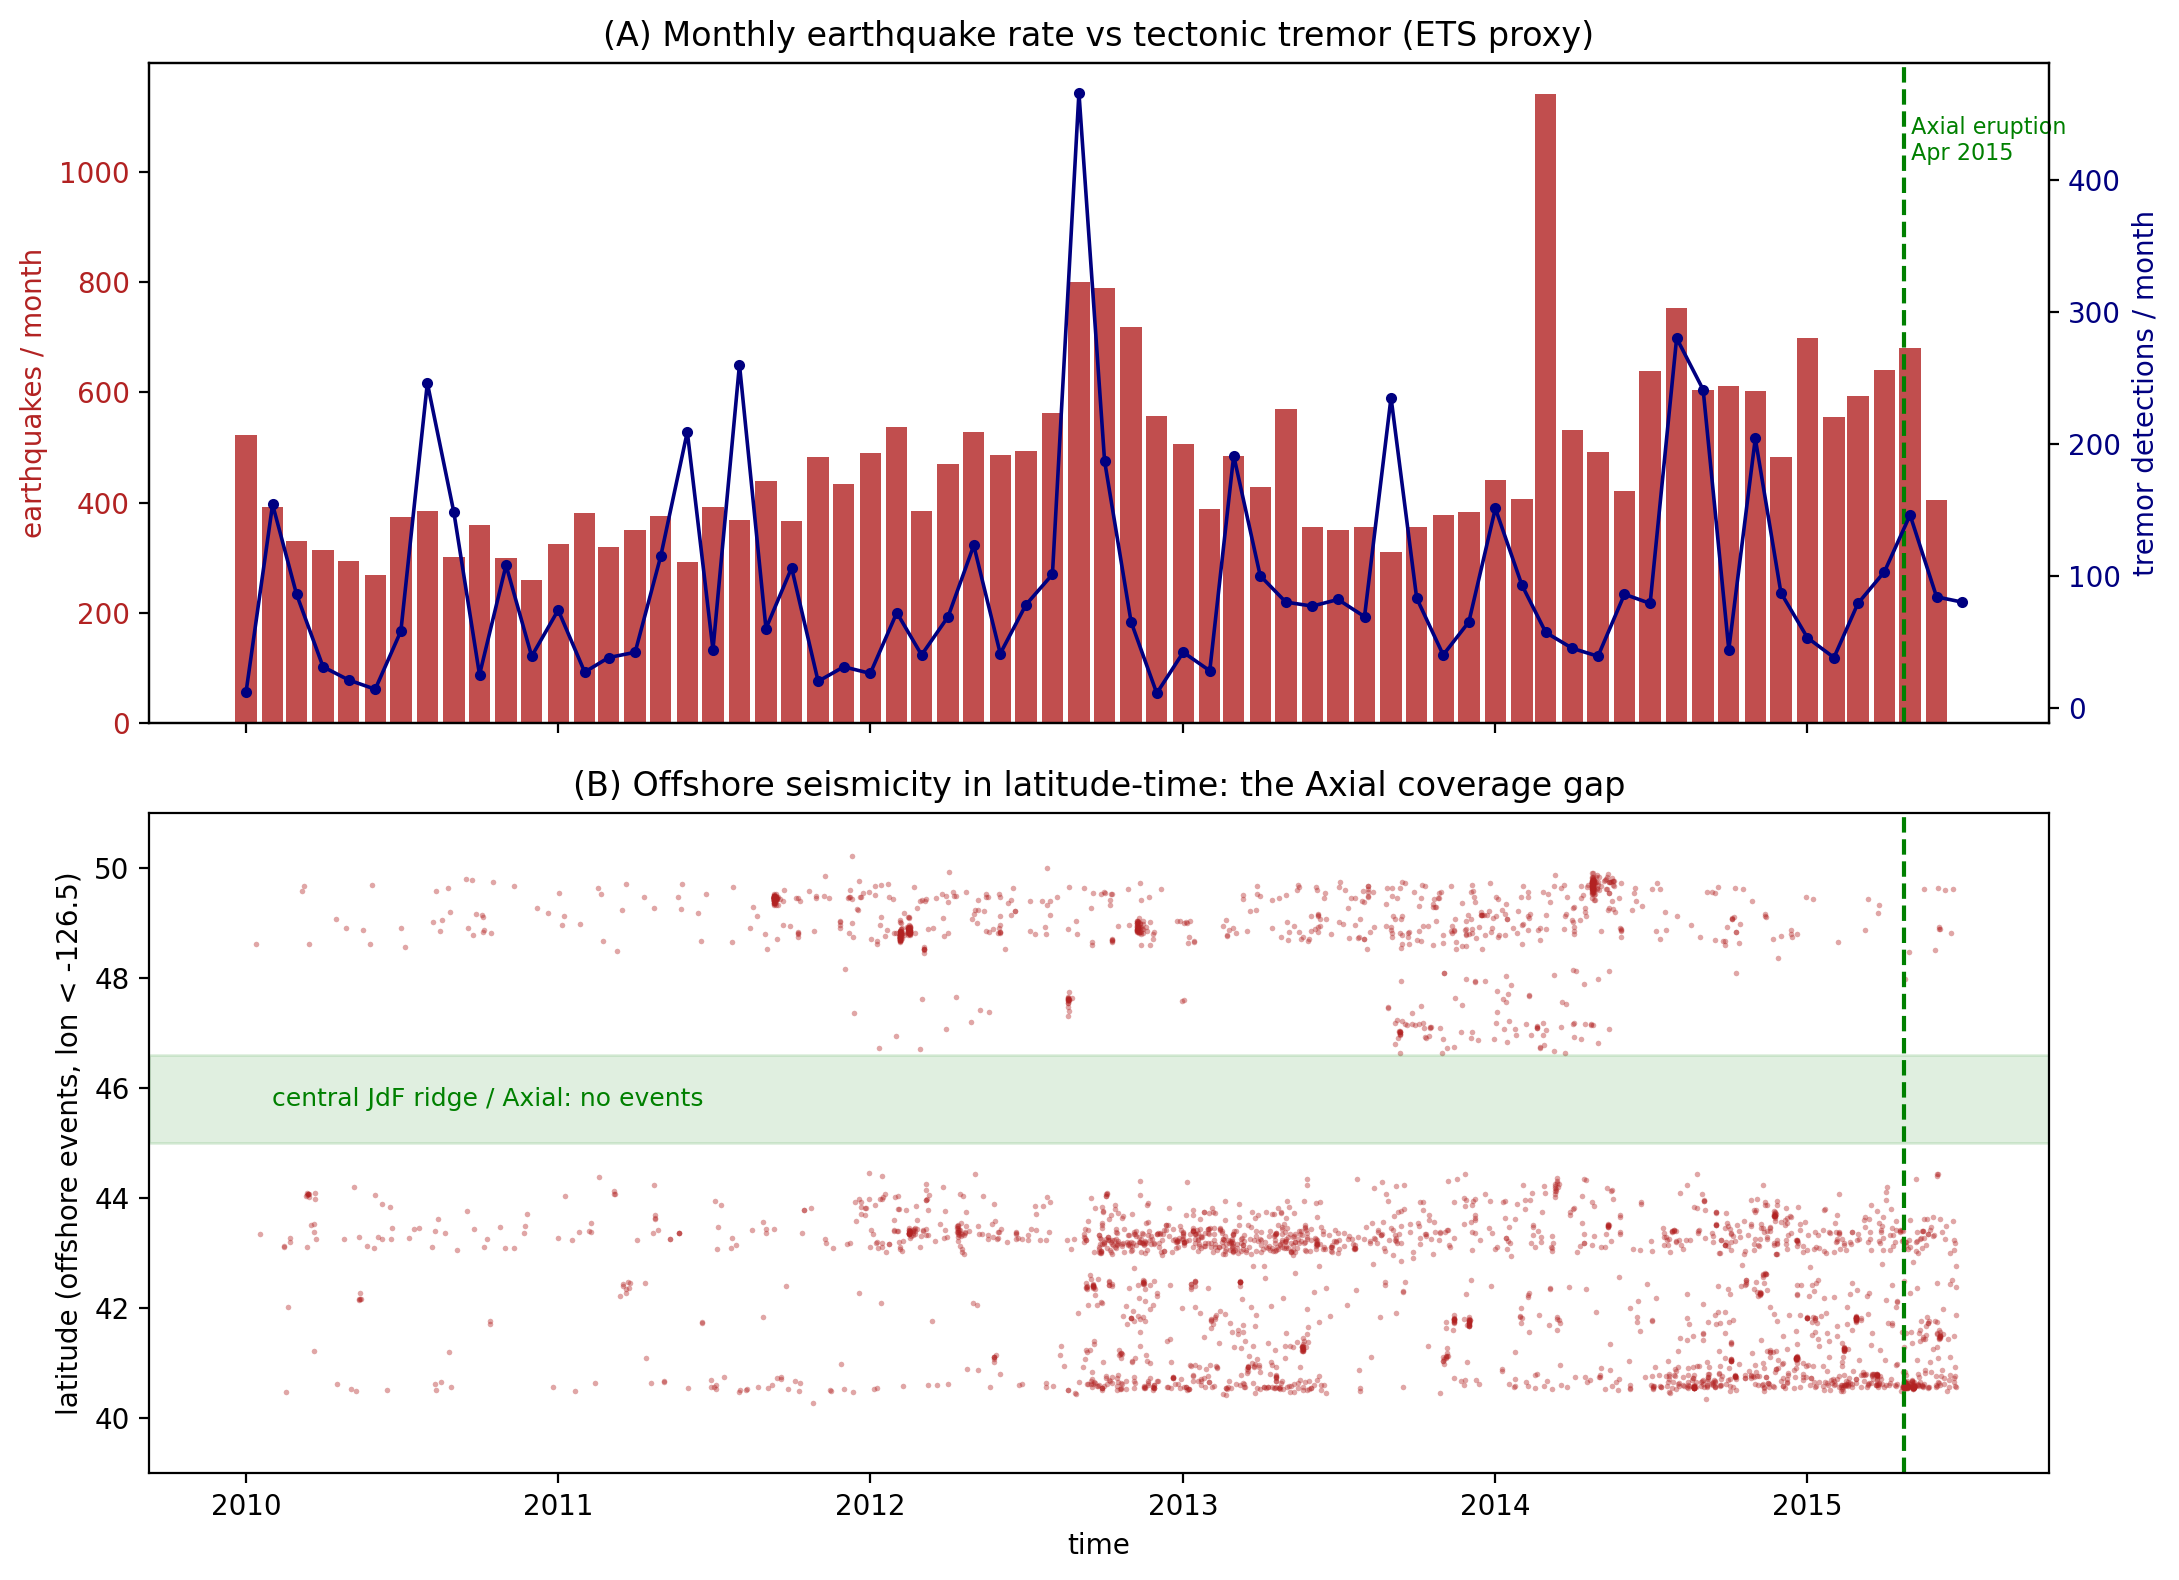
\includegraphics[width=\linewidth]{figures/supp_temporal_context.png}
    \caption{{\bf Temporal context.} (a) Monthly earthquake rate (bars) versus PNSN
    tectonic-tremor detections (line) as an ETS proxy. (b) Offshore seismicity in
    latitude--time; the shaded band marks the central JdF ridge / Axial coverage gap.}
    \label{fig:supp_temporal}
\end{figure}

\section{Event classification and location uncertainty}

Combining the interface geometry, the volcano catalog, and a horizontal location
uncertainty joined from the relocated catalog (median $\sim$4~km for the QC events),
we partition the catalog into physically distinct populations
(Figure~\ref{fig:supp_class}): volcanic (within 20~km of a Holocene edifice),
potentially megathrust (generous bucket), crustal upper-plate faults, intraslab, and
oceanic ridge/transform. Volcanic seismicity is dominated by Mount St.\ Helens
($\sim$980 events), with lesser contributions from Rainier, Hood, and submarine ridge
segments. This labeled catalog accompanies the data release.

\begin{figure}[h]
    \centering
    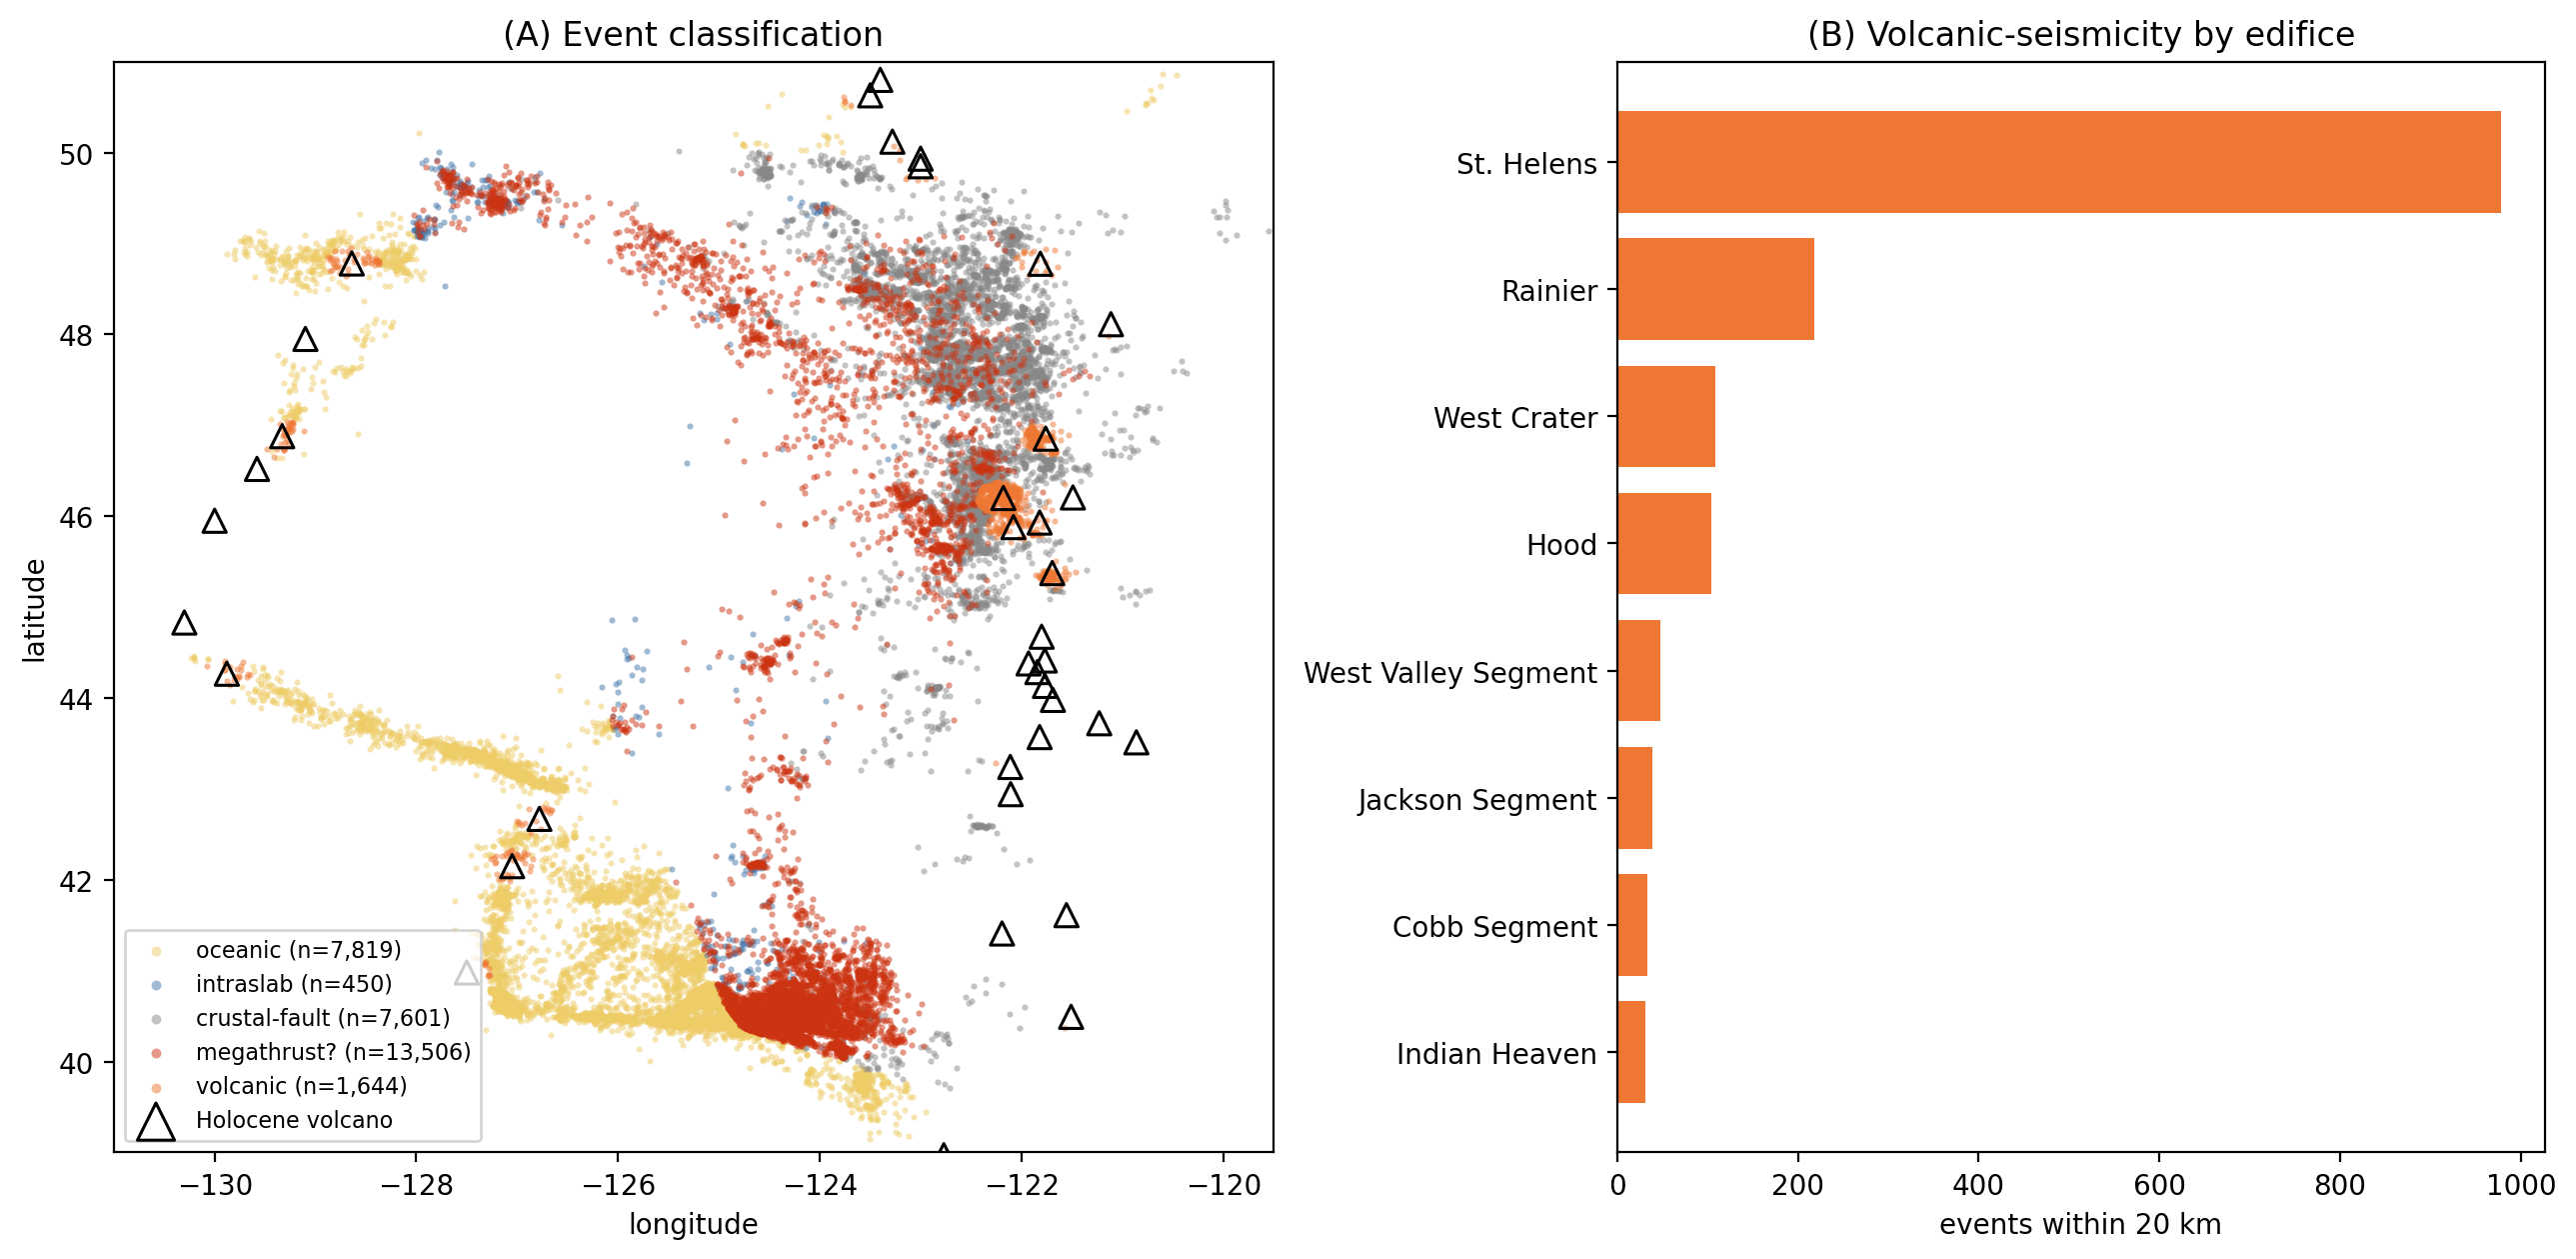
\includegraphics[width=\linewidth]{figures/supp_event_classification.png}
    \caption{{\bf Event classification.} (a) Map of the classified catalog with
    Holocene volcanoes (triangles). (b) Volcanic seismicity by edifice.}
    \label{fig:supp_class}
\end{figure}

\section{Crustal seismicity and tremor}

Using the classified crustal-fault events, the PNSN tremor catalog, and ANSS as an
independent check, we find that upper-plate crustal seismicity is largely decoupled
from the tectonic-tremor (ETS) cycle. Spatially, the crustal seismicity and tremor
occupy distinct positions (the tremor lies downdip); temporally, the monthly crustal
earthquake rate correlates only weakly with the tremor rate in both our catalog and
ANSS (Pearson $r\approx0.15$; Figure~\ref{fig:supp_tremor}), as expected for
upper-plate faulting that is not driven by slow slip on the interface.

\begin{figure}[h]
    \centering
    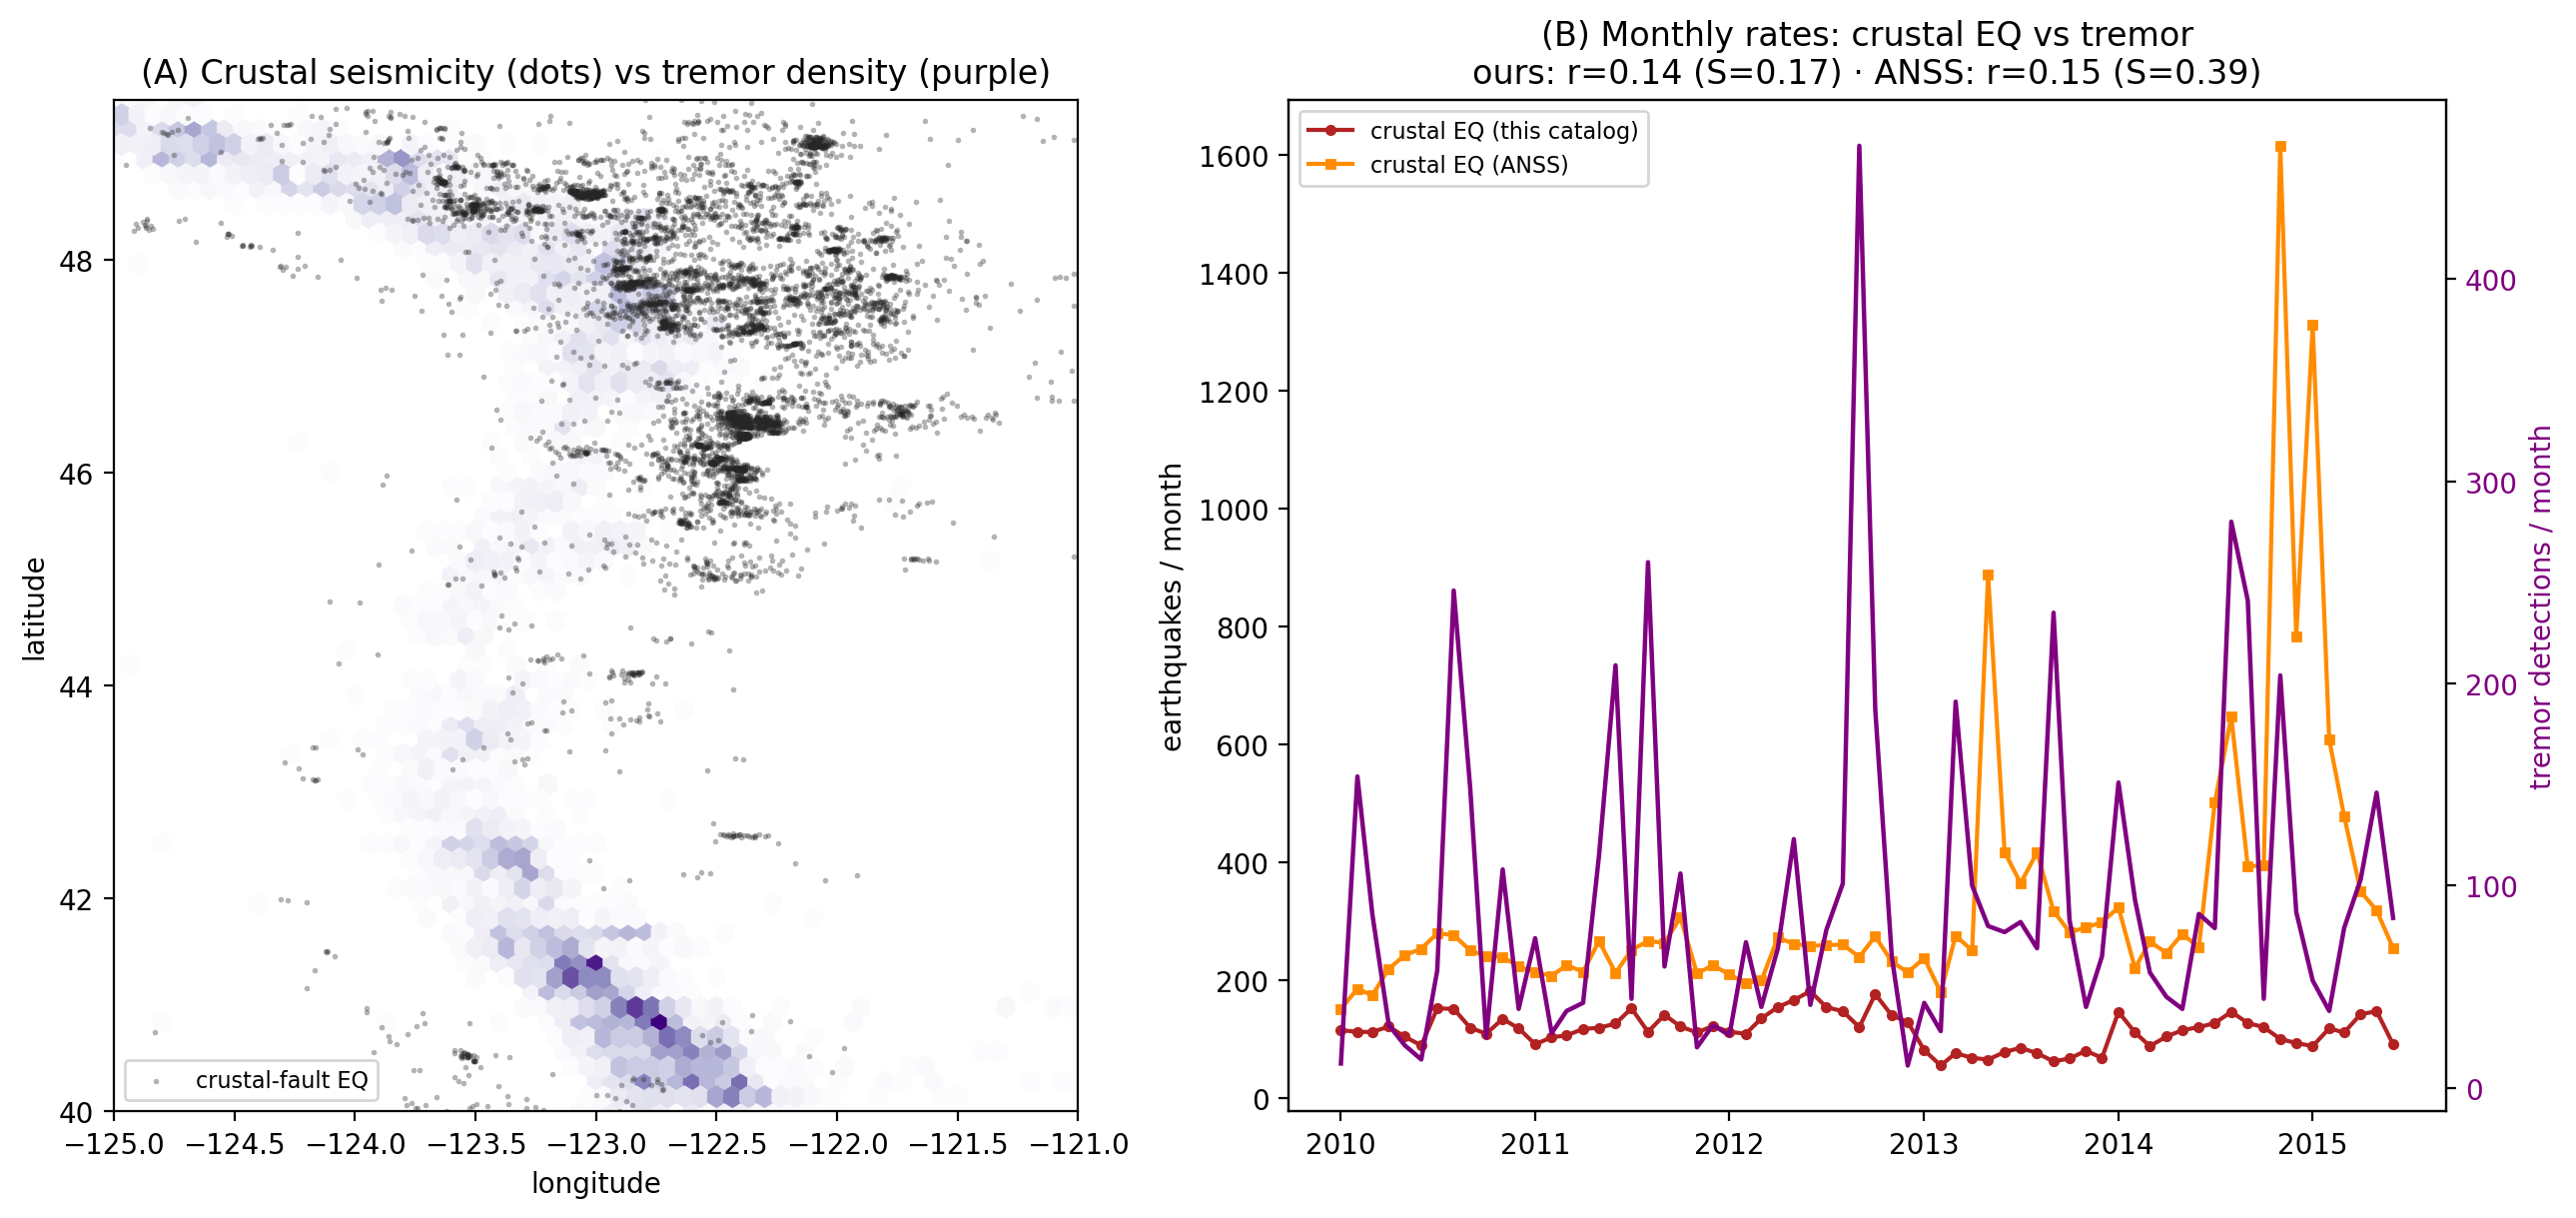
\includegraphics[width=\linewidth]{figures/supp_tremor_crustal.png}
    \caption{{\bf Crustal seismicity vs tremor.} (a) Crustal-fault events (dots) over
    tremor density (purple). (b) Monthly crustal earthquake rate (this catalog and
    ANSS) versus tremor detections, with correlation coefficients.}
    \label{fig:supp_tremor}
\end{figure}

\section{Seismicity and subducting-plate roughness}

Using seafloor bathymetric roughness (the local standard deviation of bathymetry) as a
proxy for the roughness of the incoming Juan de Fuca / Gorda plate, we find that
offshore seismicity concentrates strongly on rough seafloor: roughness sampled at
earthquake locations is about three times the random-ocean median (0.18 vs 0.05~km;
Kolmogorov--Smirnov $D=0.37$, $p<10^{-3}$; Figure~\ref{fig:supp_rough}). For the
ridge/transform events this partly reflects that the seismogenic faults \emph{are} the
rough tectonic fabric (transforms, propagator wakes, the Mendocino triple junction);
testing whether \emph{subducted} roughness modulates forearc and interface seismicity
requires projecting the incoming-plate roughness down-dip, which we leave to future work.

\begin{figure}[h]
    \centering
    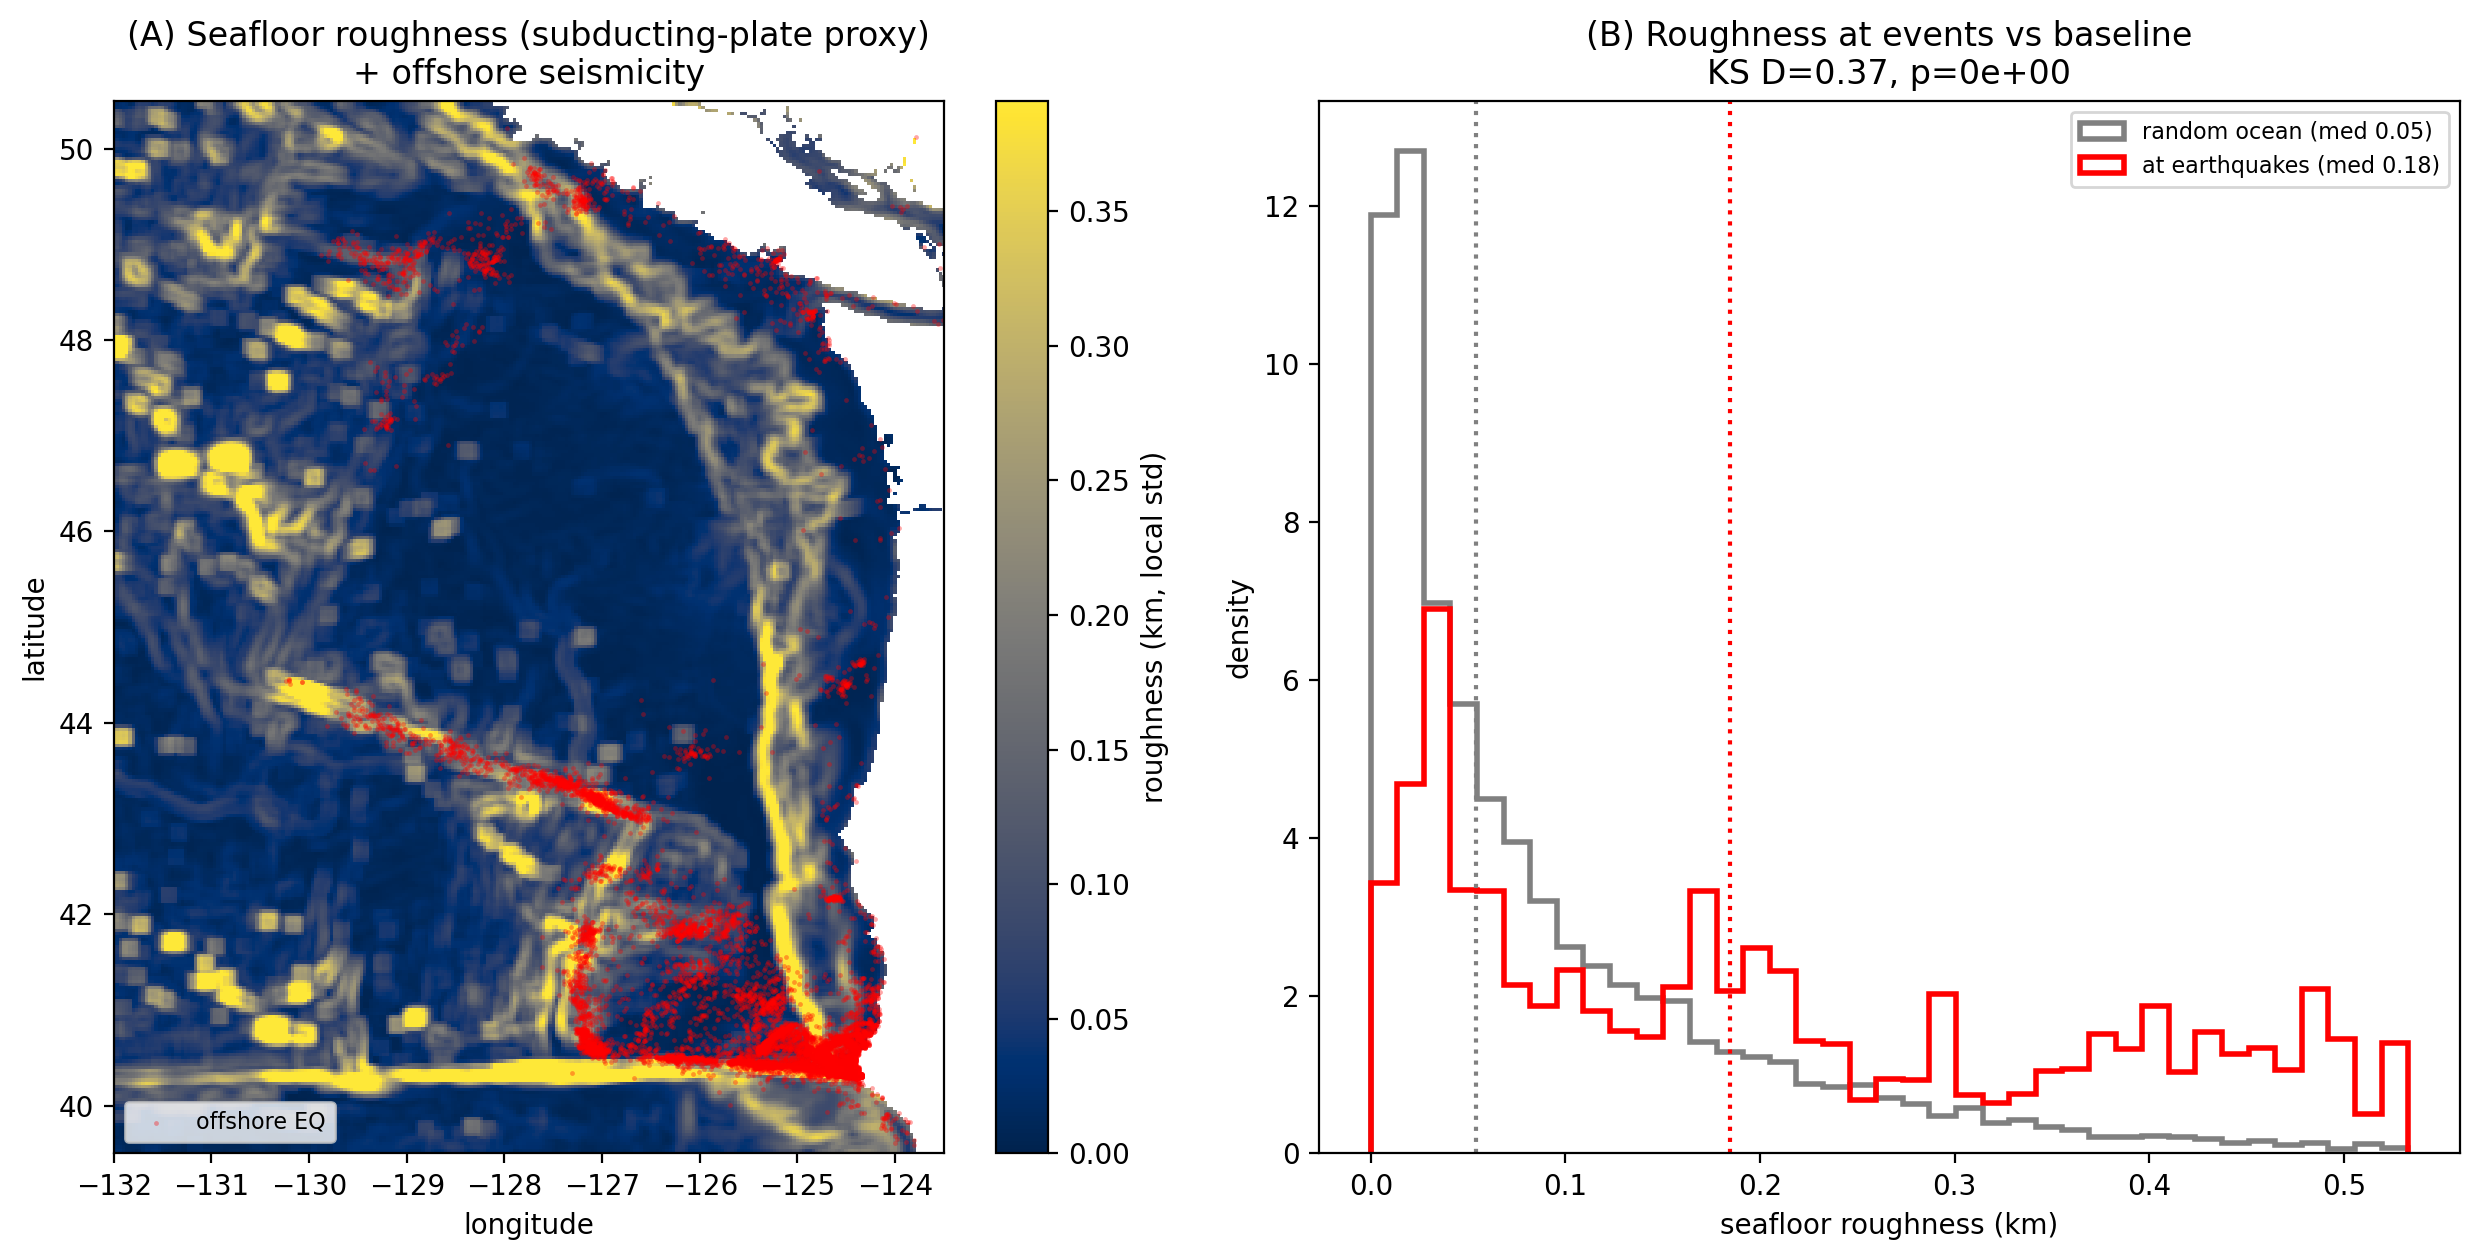
\includegraphics[width=\linewidth]{figures/supp_slab_roughness.png}
    \caption{{\bf Seismicity vs seafloor roughness.} (a) Seafloor roughness (local std
    of bathymetry) with offshore seismicity (red). (b) Roughness sampled at earthquakes
    versus a random ocean baseline.}
    \label{fig:supp_rough}
\end{figure}

\section{Seismicity and 3-D velocity structure}

We test the relation between the catalog and the Delph et al. (2018) 3-D shear-velocity
model of the Cascadia forearc \citep{Delph18} by sampling, at each event, the velocity
perturbation dlnVs from the depth-mean (positive = fast, e.g. the cold slab; negative =
slow, e.g. fluid/melt-rich mantle wedge). The classes occupy statistically distinct
velocity structure (Kolmogorov--Smirnov $p<10^{-3}$ for every class;
Figure~\ref{fig:supp_tomo}): the generous megathrust bucket concentrates in
\emph{low}-velocity material ($-2.6\%$ median), consistent with a fluid-rich plate
interface, whereas crustal-fault, volcanic, and intraslab events sit in \emph{faster}
material ($\sim+3\%$), i.e. competent crust and cold subducting lithosphere. In the
Puget Sound cross-section the interface-depth seismicity follows a down-dip low-velocity
band. This independent geophysical dataset corroborates the depth-based classification
and the fluid-control interpretation of \citet{Delph18}.

\begin{figure}[h]
    \centering
    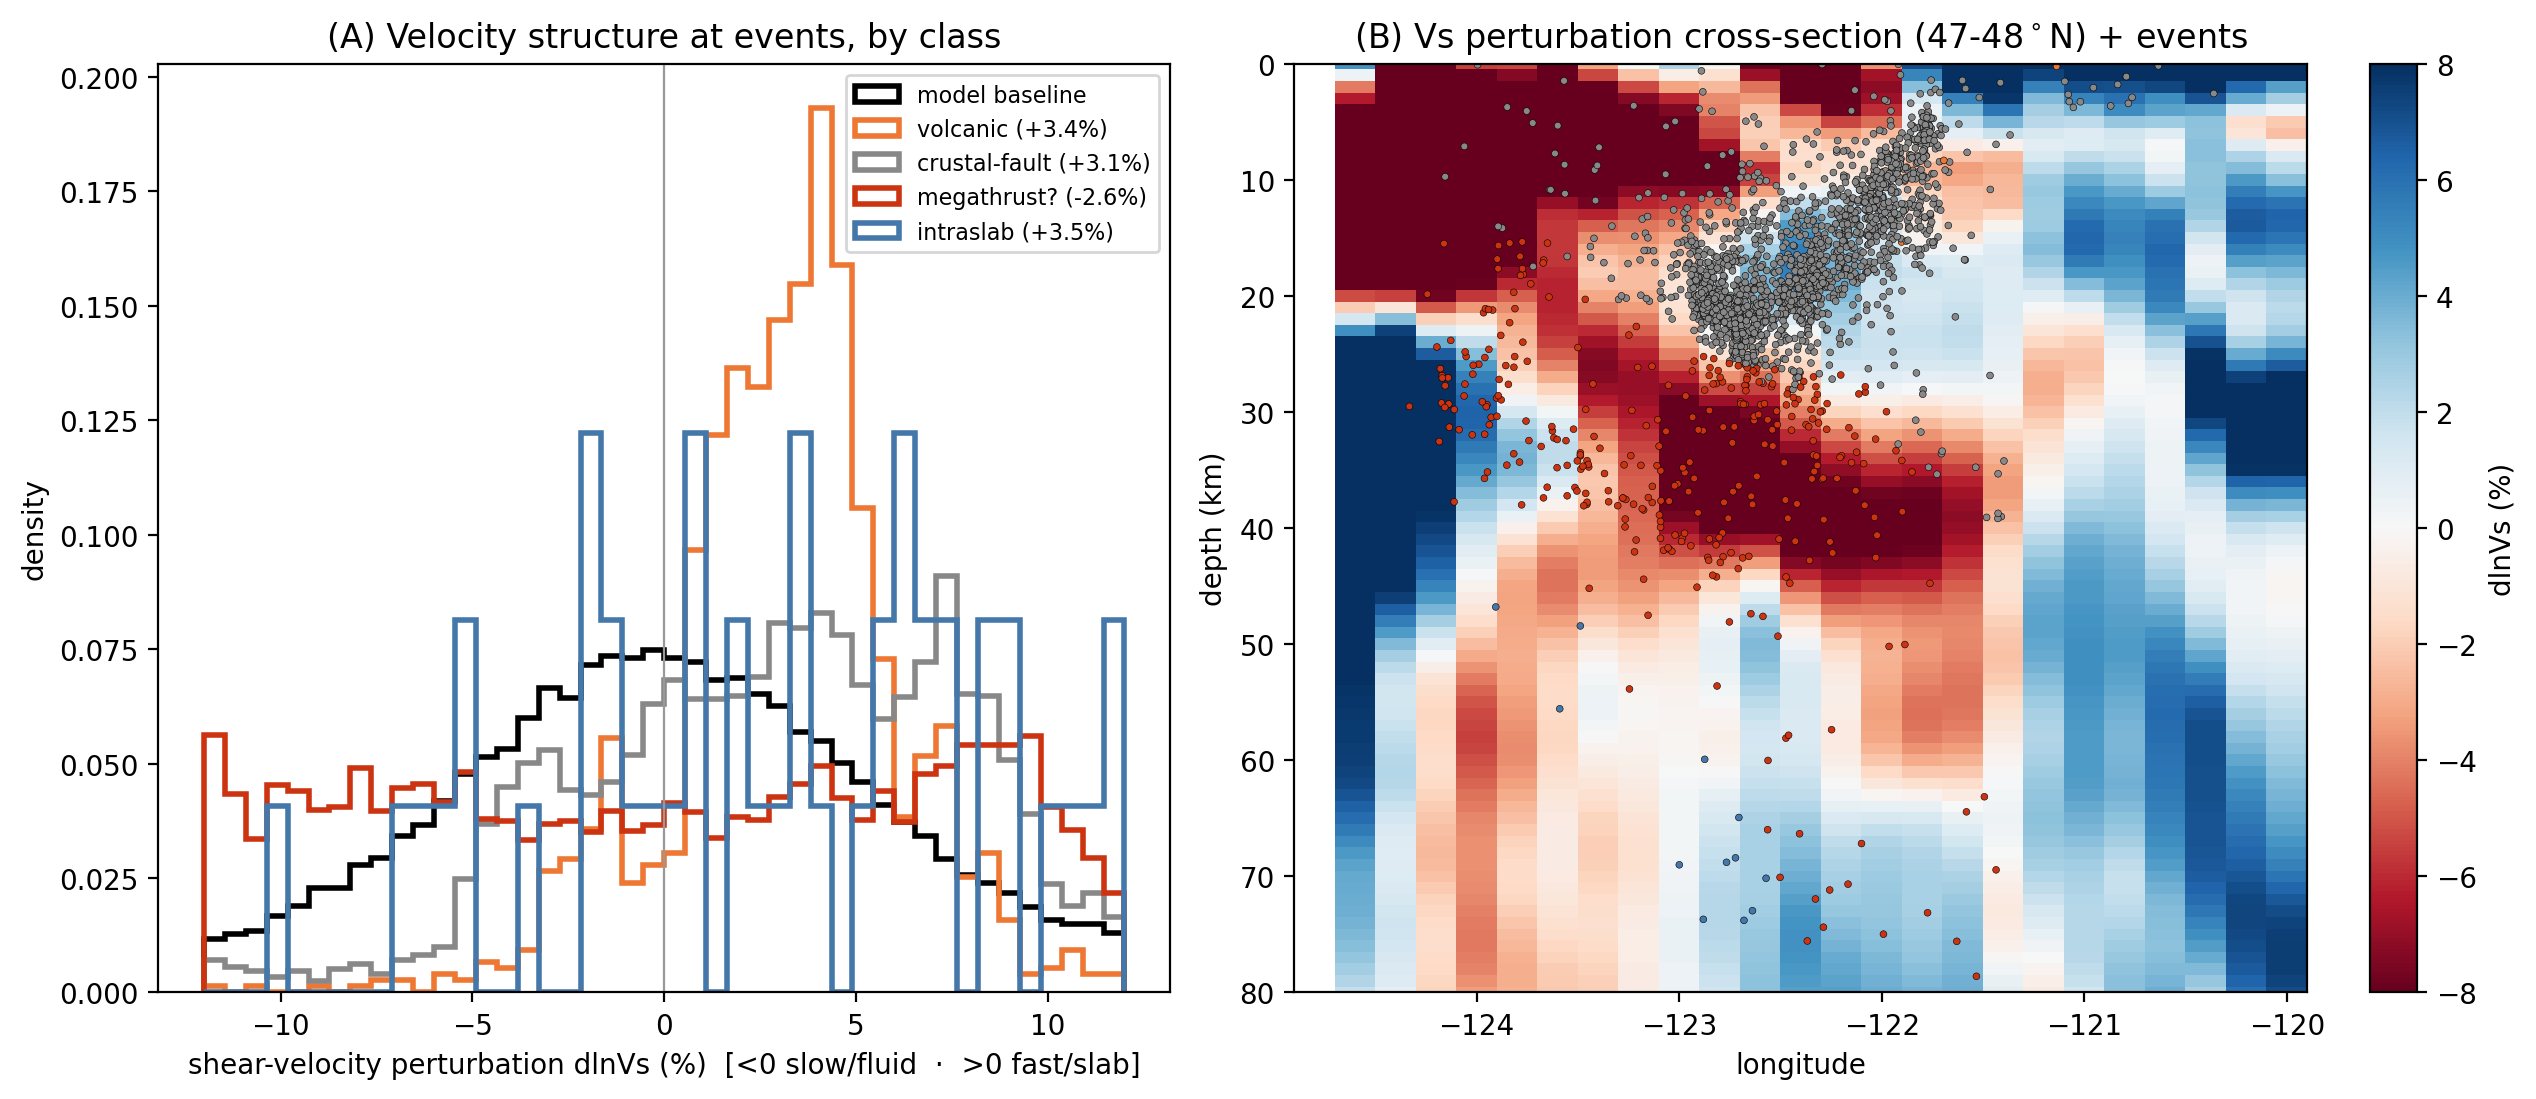
\includegraphics[width=\linewidth]{figures/supp_tomography.png}
    \caption{{\bf Seismicity vs 3-D shear velocity} \citep{Delph18}. (a) Distribution of
    velocity perturbation dlnVs at events by class, against the whole-model baseline.
    (b) Vs-perturbation cross-section (47--48$^\circ$N) with events colored by class;
    megathrust-bucket events track the down-dip low-velocity (fluid) band.}
    \label{fig:supp_tomo}
\end{figure}

\section*{Competing interests}
The authors declare no competing interests.

\bibliography{mybibfile}
    
\end{document}

